\section{Model Description}


	\subsection{Derivation of Equations of Motion - Newtonian Mechanics}

\begin{figure}[H]
	\centering
	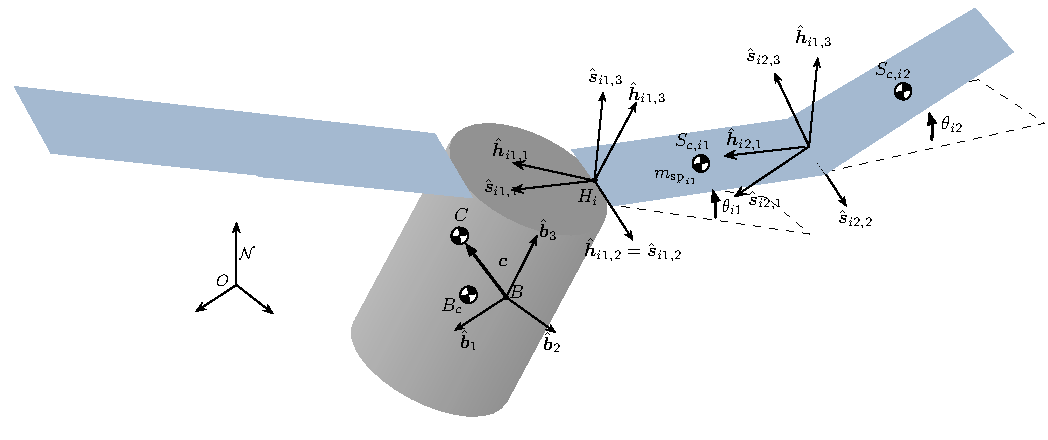
\includegraphics[]{Figures/Flex_Slosh_Figure}
	\caption{Frame and variable definitions used for formulation}
	\label{fig:Flex_Slosh_Figure}
\end{figure} 

\subsubsection{Rigid Spacecraft Hub Translational Motion}

Following a similar derivation as in previous work \cite{Allard2016rz}, the derivation begins with Newton's second law for the center of mass of the spacecraft.
\begin{equation}
	\ddot{\bm r}_{C/N} = \frac{\bm{F}}{m_{\text{\text{sc}}}}
	\label{eq:Newtons1Law}
\end{equation}
Ultimately the acceleration of the body frame or point $B$ is desired
\begin{equation}
	\ddot{\bm r}_{B/N} = \ddot{\bm r}_{C/N}-\ddot{\bm c}
	\label{eq:RcRbacc}
\end{equation}
The definition of $\bm{c}$ can be seen in Eq. (\ref{eq:c}).
\begin{equation}
	\bm{c} = \frac{1}{m_{\text{sc}}}\Big(m_{\text{\text{hub}}}\bm{r}_{B_{c}/B} + \sum_{j=1}^{N_{P}}m_j\bm{r}_{P_{c,j}/B}\Big)
	\label{eq:c} 
\end{equation}
To find the inertial time derivative of $\bm{c}$, it is first necessary to find the time derivative of $\bm{c}$ with respect to the body frame. A time derivative of any vector, $\bm{v}$, with respect to the body frame is denoted by $\bm{v}'$; the inertial time derivative is labeled as $\dot{\bm{v}}$. The first and second body-relative time derivatives of $\bm{c}$ can be seen in Eqs. (\ref{eq:cprime}) and (\ref{eq:cdprime}).

$\bm{r}_{P_{c,j}/B}$ is defined in the following
\begin{equation}
	\bm{r}_{P_{c,j}/B} = \bm{r}_{P_{j}/B} + \rho_j \hat{\bm p}_j 
\end{equation}
And, the first and second body time derivatives of $\bm{r}_{P_{c,j}/B}$ are
\begin{align}
	\bm{r}'_{P_{c,j}/B} &= \dot{\rho}_j \hat{\bm p}_j 
	\\
	\bm{r}''_{P_{c,j}/B} &= \ddot{\rho}_j \hat{\bm p}_j 
\end{align}
$\bm{c}'$ and $\bm{c}''$ are defined in the following equations
\begin{equation}
	\bm{c}' = \frac{1}{m_{\text{sc}}}\sum_{j=1}^{N_{P}}m_j\dot{\rho}_j \hat{\bm p}_j
	\label{eq:cprime}
\end{equation}
\begin{equation}
	\bm{c}'' = \frac{1}{m_{\text{sc}}}\sum_{j=1}^{N_{P}}m_j\ddot{\rho}_j \hat{\bm p}_j
	\label{eq:cdprime}
\end{equation}
Using the transport theorem\cite{schaub} yields the following definition for $\ddot{\bm c}$
\begin{equation}
	\ddot{\bm c} = \bm{c}'' + 2\bm\omega_{\cal B/N}\times\bm{c}'+\dot{\bm\omega}_{\cal B/N}\times\bm{c}+\bm\omega_{\cal B/N}\times\left(\bm\omega_{\cal B/N}\times\bm{c}\right)
	\label{eq:cddot}
\end{equation}
Eq.~\eqref{eq:RcRbacc} is updated to include Eq.~\eqref{eq:cddot}
\begin{equation}
	\ddot{\bm r}_{B/N} = \ddot{\bm r}_{C/N}-\bm{c}'' - 2\bm\omega_{\cal B/N}\times\bm{c}'-\dot{\bm\omega}_{\cal B/N}\times\bm{c}-\bm\omega_{\cal B/N}\times\left(\bm\omega_{\cal B/N}\times\bm{c}\right)
	\label{eq:Rbddot}
\end{equation}
Substituting Eq.\eqref{eq:cdprime} into Eq.\eqref{eq:Rbddot} results in
\begin{equation}
	\ddot{\bm r}_{B/N} = \ddot{\bm r}_{C/N}-\frac{1}{m_{\text{sc}}}\sum_{j=1}^{N_{P}}m_j\ddot{\rho}_j \hat{\bm p}_j = 
	- 2\bm\omega_{\cal B/N}\times\bm c'
	-\dot{\bm\omega}_{\cal B/N}\times\bm{c}-\bm\omega_{\cal B/N}\times\left(\bm\omega_{\cal B/N}\times\bm{c}\right)
	\label{eq:Rbddot2}
\end{equation}
Moving second order terms to the left hand side and introducing the tilde matrix\cite{schaub} to replace the cross product operators simplifies the equation to
\begin{equation}
	m_{\text{sc}} \ddot{\bm r}_{B/N}-m_{\text{sc}} [\tilde{\bm{c}}] \dot{\bm\omega}_{\cal B/N} +\sum_{j=1}^{N_{P}}m_j \hat{\bm p}_j \ddot{\rho}_j = \bm F_{\text{ext}}	- 2 m_{\text{sc}} [\tilde{\bm\omega}_{\cal B/N}] \bm c'
	- m_{\text{sc}} [\tilde{\bm\omega}_{\cal B/N}][\tilde{\bm\omega}_{\cal B/N}]\bm{c}
	\label{eq:Rbddot3}
\end{equation}

Equation~\eqref{eq:Rbddot3} is the translational motion equation and is the first EOM needed to describe the motion of the spacecraft. The following section develops the rotational EOM.

\subsubsection{Rigid Spacecraft Hub Rotational Motion}

Starting with Euler's equation when the body fixed coordinate frame origin is not coincident with the center of mass of the body\cite{schaub}
\begin{equation}
	\bm{\dot{H}}_{\text{sc},B} = \bm{L}_B+m_{\text{\text{sc}}}\ddot{\bm r}_{B/N}\times\bm{c}
	\label{eq:Euler}
\end{equation}
where $\bm{L}_B$ is the total external torque about point $B$. The definition of the angular momentum vector of the spacecraft about point $B$ is
\begin{equation}
	\bm{H}_{\text{sc},B} = [I_{\text{hub},B_c}] \bm\omega_{\cal B/N} + m_{\text{\text{hub}}}\bm{r}_{B_{c}/B} \times \dot{\bm{r}}_{B_{c}/B} + \sum\limits_{j=1}^{N_P}m_j \bm r_{P_{c,j}/B}\times \dot{\bm r}_{P_{c,j}/B}
	\label{eq:Hb2}
\end{equation}

Now the inertial time derivative of Eq. \eqref{eq:Hb2} is taken and yields
\begin{equation}
	\dot{\bm{H}}_{\text{sc},B} = [I_{\text{hub},B_c}] \dot{\bm\omega}_{\cal B/N} + \bm\omega_{\cal B/N} \times [I_{\text{hub},B_c}] \bm\omega_{\cal B/N} + m_{\text{\text{hub}}}\bm{r}_{B_{c}/B} \times \ddot{\bm{r}}_{B_{c}/B} +  \sum\limits_{j=1}^{N_P}m_j \bm r_{P_{c,j}/B}\times \ddot{\bm r}_{P_{c,j}/B}
	\label{eq:Hbdot}
\end{equation}
$\ddot{\bm r}_{P_{c,j}/B}$ is
\begin{align}
	\ddot{\bm{r}}_{P_{c,j}/B}  &= \bm{r}''_{P_{c,j}/B} +2 \bm\omega_{\cal B/N} \times \bm{r}'_{P_{c,j}/B} + \dot{\bm\omega}_{\cal B/N} \times \bm{r}_{P_{c,j}/B}  +\bm\omega_{\cal B/N} \times (\bm\omega_{\cal B/N} \times \bm{r}_{P_{c,j}/B})
	\label{eq:rpddot}
\end{align}
Incorporating Eq.-~\eqref{eq:rpddot} into Eq.~\eqref{eq:Hbdot} results in
\begin{multline}
	\dot{\bm{H}}_{\text{sc},B} = [I_{\text{hub},B_c}] \dot{\bm\omega}_{\cal B/N} + \bm\omega_{\cal B/N} \times [I_{\text{hub},B_c}] \bm\omega_{\cal B/N} + m_{\text{\text{hub}}}\bm{r}_{B_{c}/B} \times \ddot{\bm{r}}_{B_{c}/B}\\ + \sum\limits_{j=1}^{N_P}m_j \bm r_{P_{c,j}/B}\times \Bigl[\bm{r}''_{P_{c,j}/B} +2 \bm\omega_{\cal B/N} \times \bm{r}'_{P_{c,j}/B} + \dot{\bm\omega}_{\cal B/N} \times \bm{r}_{P_{c,j}/B} +\bm\omega_{\cal B/N} \times (\bm\omega_{\cal B/N} \times \bm{r}_{P_{c,j}/B})\Bigr]
	\label{eq:Hbdot2}
\end{multline}
Applying the parallel axis theorem the following inertia tensor terms are defined as
\begin{align}
	[I_{\text{sc},B}] &= [I_{\text{hub},B}] + m_{\text{hub}} [\tilde{\bm{r}}_{B_{c}/B}] [\tilde{\bm{r}}_{B_{c}/B}]^T + \sum\limits_{j=1}^{N_P} m_j [\tilde{\bm{r}}_{P_{c,j}/B}] [\tilde{\bm{r}}_{P_{c,j}/B}]^T
	\label{eq:IscB}
\end{align}
Taking the body-relative time derivative of Equation~\eqref{eq:IscB} yields
\begin{equation}
	[I'_{\text{sc},B}] =
	- \sum\limits_{j=1}^{N_P} m_j \Bigl(  [\tilde{\bm{r}}'_{P_{c,j}/B}] [\tilde{\bm{r}}_{P_{c,j}/B}] + [\tilde{\bm{r}}_{P_{c,j}/B}] [\tilde{\bm{r}}'_{P_{c,j}/B}]  \Bigr)
\end{equation}
The Jacobi Identity, $(\bm a \times \bm b)\times \bm c = \bm a \times (\bm b\times \bm c) - \bm b \times (\bm a\times \bm c)$, is used to combine terms and produce the following simplified equation
\begin{multline}
	\dot{\bm{H}}_{\text{sc},B} = [I_{\text{sc},B}] \dot{\bm\omega}_{\cal B/N} + \bm\omega_{\cal B/N} \times [I_{\text{sc},B}] \bm\omega_{\cal B/N} + [I'_{\text{sc},B}] \bm\omega_{\cal B/N}
	\\+ \sum\limits_{j=1}^{N_P}\biggl[m_j \bm r_{P_{c,j}/B}\times\bm{r}''_{P_{c,j}/B}
	+ m_j \bm\omega_{\cal B/N} \times \Bigl(\bm{r}_{P_{c,j}/B} \times \bm{r}'_{P_{c,j}/B}\Bigr)\biggr]
	\label{eq:Hbdot4}
\end{multline}

Eqs. (\ref{eq:Euler}) and (\ref{eq:Hbdot4}) are equated and yield
\begin{multline}
	\bm{L}_B+m_{\text{sc}}\ddot{\bm r}_{B/N}\times\bm{c} = [I_{\text{sc},B}] \dot{\bm\omega}_{\cal B/N} + \bm\omega_{\cal B/N} \times [I_{\text{sc},B}] \bm\omega_{\cal B/N} + [I'_{\text{sc},B}] \bm\omega_{\cal B/N}
	\\+ \sum\limits_{j=1}^{N_P}\biggl[m_j \bm r_{P_{c,j}/B}\times\bm{r}''_{P_{c,j}/B}
	+ m_j \bm\omega_{\cal B/N} \times \Bigl(\bm{r}_{P_{c,j}/B} \times \bm{r}'_{P_{c,j}/B}\Bigr)\biggr]
	\label{eq:Hbdot5}
\end{multline}
Finally, using tilde matrix and simplifying yields the modified Euler equation, which is the second EOM necessary to describe the motion of the spacecraft.
\begin{multline}
	[I_{\text{sc},B}] \dot{\bm\omega}_{\cal B/N} = -[\bm{\tilde{\omega}}_{\cal B/N}] [I_{\text{sc},B}] \bm\omega_{\cal B/N} - [I'_{\text{sc},B}] \bm\omega_{\cal B/N}	\\- \sum\limits_{j=1}^{N_P}\biggl(m_j [\tilde{\bm r}_{P_{c,j}/B}]\bm{r}''_{P_{c,j}/B}
	+ m_j [\tilde{\bm\omega}_{\cal B/N}] [\tilde{\bm{r}}_{P_{c,j}/B}] \bm{r}'_{P_{c,j}/B}\biggr) 
	+ \bm{L}_B - m_{\text{sc}} [\tilde{\bm{c}}] \ddot{\bm r}_{B/N}
	\label{eq:Final5}
\end{multline}
Rearranging Eq.~\eqref{eq:Final5} to be in the same form as the previous sections results in
\begin{multline}
	m_{\text{sc}}[\tilde{\bm{c}}]\ddot{\bm r}_{B/N}+[I_{\text{sc},B}] \dot{\bm\omega}_{\cal B/N} + \sum\limits_{j=1}^{N_P}m_j [\tilde{\bm r}_{P_{c,j}/B}] \hat{\bm p}_j \ddot{\rho}_j = \\
	-[\bm{\tilde{\omega}}_{\cal B/N}] [I_{\text{sc},B}] \bm\omega_{\cal B/N} 
	- [I'_{\text{sc},B}] \bm\omega_{\cal B/N} 	- \sum\limits_{j=1}^{N_P} m_j [\tilde{\bm\omega}_{\cal B/N}] [\tilde{\bm{r}}_{P_{c,j}/B}] \bm{r}'_{P_{c,j}/B} + \bm{L}_B
	\label{eq:Final6}
\end{multline} 

\subsubsection{Fuel Slosh Motion}
Figure~\ref{fig:Flex_Slosh_Figure} shows that a single fuel slosh particle is free to move along its corresponding $\hat{\bm p}_j$ direction and this formulation is generalized to include $N_P$ number of fuel slosh particles. The derivation begins with Newton's law for each fuel slosh particle:
\begin{equation}
	m_j \ddot{\bm{r}}_{P_{c,j}/N} = \bm F_G + \bm F_C- k_j \rho_j \hat{\bm p}_j - c_j \dot{\rho_j} \hat{\bm p}_j
	\label{eq:sloshaccel}
\end{equation}
Where $\bm F_C$ is the constraint force that maintains the fuel slosh mass to travel along the direction $\hat{\bm p}_j$. The forces due to the spring and damper are explicitly included in Eq.~\eqref{eq:sloshaccel} and result in a restoring force and damping force. $\ddot{\bm{r}}_{P_{c,j}/N}$ is defined in the following equation.
\begin{equation}
	\ddot{\bm{r}}_{P_{c,j}/N} = \ddot{\bm{r}}_{B/N} + \ddot{\bm{r}}_{P_{c,j}/B}
\end{equation}
The inertial acceleration vector $\ddot{\bm{r}}_{P_{c,j}/B}$ is defined in Eq.~\eqref{eq:rpddot}. Plugging this definition into Eq.~\eqref{eq:sloshaccel} results in
\begin{multline}
	m_j \Big[\ddot{\bm{r}}_{B/N} + \ddot{\rho}_j \hat{\bm p}_j  +2 \bm\omega_{\cal B/N} \times \bm{r}'_{P_{c,j}/B} + \dot{\bm\omega}_{\cal B/N} \times \bm{r}_{P_{c,j}/B}  +\bm\omega_{\cal B/N} \times (\bm\omega_{\cal B/N} \times \bm{r}_{P_{c,j}/B})\Big]\\
	=  \bm F_G + \bm F_C - k_j \rho_j \hat{\bm p}_j - c_j \dot{\rho_j} \hat{\bm p}_j
	\label{eq:sloshaccel3}
\end{multline}	

Equation~\eqref{eq:sloshaccel3} is the dynamical equation for a fuel slosh particle, however, the constraint force, $\bm F_C$, is undefined. Since the fuel slosh particle is free to move in the $\hat{\bm p_j}$ direction, the component of $\bm F_C$ along the $\hat{\bm p_j}$ direction is zero. Leveraging this insight, Eq.~\eqref{eq:sloshaccel3} is projected into the $\hat{\bm p_j}$ direction by multiplying both sides of the equation by $\hat{\bm p_j}^T$.
\begin{multline}
	m_j \Bigl(\hat{\bm p_j}^T \ddot{\bm{r}}_{B/N} + \ddot{\rho}_j  +2 \hat{\bm p_j}^T  \bm\omega_{\cal B/N} \times \bm{r}'_{P_{c,j}/B} + \hat{\bm p_j}^T \dot{\bm\omega}_{\cal B/N} \times \bm{r}_{P_{c,j}/B}  + \hat{\bm p_j}^T \bm\omega_{\cal B/N} \times (\bm\omega_{\cal B/N} \times \bm{r}_{P_{c,j}/B})\Bigr)\\
	= \hat{\bm p_j}^T \bm F_G - k_j \rho_j - c_j \dot{\rho_j}
	\label{eq:sloshaccel4}
\end{multline}	
Moving the second order terms to the left hand side and introducing the tilde matrix notation yields the final equation needed to describe the motion of the spacecraft.
\begin{multline}
	m_j \hat{\bm p_j}^T \ddot{\bm{r}}_{B/N} - m_j \hat{\bm p_j}^T [\tilde{\bm{r}}_{P_{c,j}/B}] \dot{\bm\omega}_{\cal B/N} + m_j \ddot{\rho}_j  \\
	= \hat{\bm p_j}^T \bm F_G - k_j \rho_j - c_j \dot{\rho_j} - 2 m_j \hat{\bm p_j}^T  [\tilde{\bm\omega}_{\cal B/N}] \bm{r}'_{P_{c,j}/B}  - m_j \hat{\bm p_j}^T [\tilde{\bm\omega}_{\cal B/N}] [\tilde{\bm\omega}_{\cal B/N}] \bm{r}_{P_{c,j}/B} 
	\label{eq:sloshaccel5}
\end{multline}	

\subsection{Derivation of Equations of Motion - Kane's Method}

The choice of generalized coordinates and their respective generalized speeds are:

\begin{equation}
	\bm q = 
	\begin{bmatrix}
		\bm r_{B/N}\\
		\bm \sigma_{\cal{B/N}}\\
		\rho_1\\
		\cdot\\
		\rho_{N_P}
	\end{bmatrix}
	\quad
	\bm u = \begin{bmatrix}
		\dot{\bm r}_{B/N}\\
		\bm \omega_{\cal{B/N}}\\
		\dot{\rho}_1\\
		\cdot\\
		\dot{\rho}_{N_P}
	\end{bmatrix}
\end{equation} 

The necessary velocities needed to be defined are as follows

\begin{equation}
\dot{\bm r}_{B_c/N} = \dot{\bm r}_{B/N} + \bm \omega_{\cal{B/N}} \times {\bm r}_{B_c/B} = \dot{\bm r}_{B/N}  - [\tilde{{\bm r}}_{B_c/B}] \bm \omega_{\cal{B/N}} \\
\end{equation}

\begin{equation}
	\dot{\bm r}_{C/N} = \dot{\bm r}_{B/N} + \dot{\bm c}\\
	\label{eq:rDot_CN}
\end{equation}

\begin{equation}
	\bm \omega_{\cal{B/N}} = \bm \omega_{\cal{B/N}}
\end{equation}

\begin{equation}
	\dot{\bm r}_{P_{c,j}/N} = \dot{\bm r}_{B/N} + {\bm r}'_{P_{c,j}/B} + \bm \omega_{\cal{B/N}} \times {\bm r}_{P_{c,j}/B} = \dot{\bm r}_{B/N} + \dot{\rho}_j \hat{\bm p}_j  - [\tilde{{\bm r}}_{P_{c,j}/B}] \bm \omega_{\cal{B/N}}
\end{equation}

Now the following partial velocity table can be created:

\begin{table}[htbp]
	\caption{Partial Velocity Table}
	\label{tab:hub}
	\centering \fontsize{10}{10}\selectfont
	\begin{tabular}{ c | c | c | c } % Column formatting, 
		\hline
		$r$  & $\bm v^{B_c}_{r}$  & $\bm \omega_{\textit{r}}^{\cal{B}}$ & $\bm v^{P_c}_{r}$ \\
		\hline
		$1-3$  & $[I_{3\times 3}]$ & $[0_{3\times 3}]$ & $[I_{3\times 3}]$ \\
		$4-6$ & $- [\tilde{{\bm r}}_{B_c/B}]$ & $[I_{3\times 3}]$ & $- [\tilde{{\bm r}}_{P_{c,j}/B}]$ \\
		$7-{N_P}$ &$[0_{3\times 1}]$ & $[0_{3\times 1}]$ & $\hat{\bm p}_j$ \\
		\hline
	\end{tabular}
\end{table}

An additional partial velocity that is needed is $[\bm v^C_{1-3}]$ for the external force applied on the spacecraft, $\bm F_{\text{ext}}$. Using Eq.\eqref{eq:rDot_CN} the following is defined:

\begin{equation}
	[\bm v^C_{1-3}] = [I_{3\times 3}]
\end{equation}

Using these partial velocity definitions, the follow sections will step through the formulation for the translational, rotational and slosh EOMs developed using Kane's method.

\subsubsection{Rigid Spacecraft Hub Translational Motion}

Starting with the definition of a generalized force:

\begin{equation}
	\bm F_r = \bm v_r^T \bm F
	\label{eq:genActive}
\end{equation}
Using this definition the external force applied on the spacecraft for the translational equations is defined as:

\begin{equation}
	\bm F_{1-3} = [\bm v^C_{1-3}]^T \bm F_{\text{ext}} = \bm F_{\text{ext}}
\end{equation}

Using the definition of generalized inertia forces,
\begin{equation}
	\bm F^*_r = \sum\limits_{r}^{N}\Big[\bm \omega_r^T \bm T^* +  \bm v_r^T (- m_r \bm a_r)\Big]
	\label{eq:genInert}
\end{equation}
the inertia forces for the hub translational motion are defined as

\begin{equation}
	\bm F^*_{1-3} = [\bm v^B_{1-3}]^T (-m_{\text{hub}} \ddot{\bm r}_{B_c/N}) + \sum\limits_{j}^{N_P}[\bm v^{P_c}_{1-3}]^T (-m_j \ddot{\bm r}_{P_{c,j}/N}) = -m_{\text{hub}} \ddot{\bm r}_{B_c/N} + \sum\limits_{j}^{N_P} -m_j \ddot{\bm r}_{P_{c,j}/N}
\end{equation}

Finally, Kane's equation is:

\begin{equation}
	\bm F_r + \bm F^*_r = 0
	\label{eq:KanesEq}
\end{equation}
therefore
\begin{equation}
	\bm F_{\text{ext}} -m_{\text{hub}} \ddot{\bm r}_{B_c/N} + \sum\limits_{j}^{N_P} -m_j \ddot{\bm r}_{P_{c,j}/N} = 0
\end{equation}
Expanding and rearranging results in
\begin{equation}
	m_{\text{hub}} \ddot{\bm r}_{B_c/N} + \sum\limits_{j}^{N_P} m_j (\ddot{\bm r}_{B/N} + \ddot{\bm r}_{P_{c,j}/B}) = \bm F_{\text{ext}}
	\label{eq:KanesTrans}
\end{equation}
Plugging Eq.~\eqref{eq:rpddot} into Eq.~\eqref{eq:KanesTrans} results in
\begin{multline}
	m_{\text{hub}} (\ddot{\bm r}_{B_c/N} + \ddot{\bm r}_{B_c/B}) + \sum\limits_{j}^{N_P} m_j \Big[\ddot{\bm r}_{B/N} + \ddot{\rho}_j \hat{\bm p}_j  +2 \bm\omega_{\cal B/N} \times \bm{r}'_{P_{c,j}/B} + \dot{\bm\omega}_{\cal B/N} \times \bm{r}_{P_{c,j}/B}  \\
	+\bm\omega_{\cal B/N} \times (\bm\omega_{\cal B/N} \times \bm{r}_{P_{c,j}/B})\Big] = \bm F_{\text{ext}}
\end{multline}
Combining like terms and rearranging results in
\begin{equation}
	m_{\text{sc}} \ddot{\bm r}_{B/N}-m_{\text{sc}} [\tilde{\bm{c}}] \dot{\bm\omega}_{\cal B/N} +\sum_{j=1}^{N_{P}}m_j \hat{\bm p}_j \ddot{\rho}_j = \bm F_{\text{ext}}	- 2 m_{\text{sc}} [\tilde{\bm\omega}_{\cal B/N}] \bm c'
	- m_{\text{sc}} [\tilde{\bm\omega}_{\cal B/N}][\tilde{\bm\omega}_{\cal B/N}]\bm{c}
	\label{eq:Rbddot4}
\end{equation}
Which is identical to Eq.~\eqref{eq:Rbddot3} found using Newtonian mechanics.
\subsubsection{Rigid Spacecraft Hub Rotational Motion}

The torque acting on the spacecraft, $\bm L_B$ needs to be defined as a general active force. Using Eq.~\eqref{eq:genActive} active forces acting on the spacecraft for the rotational equations can be defined as:

\begin{equation}
	\bm F_{4-6} = [\bm \omega_{4-6}^{\cal{B}}]^T \bm L_B = \bm L_B
\end{equation}

To define the generalized inertia forces, using Eq.~\eqref{eq:genInert} the definition of $\bm T^*$ needs to be defined for a rigid body and applying it to the hub:

\begin{equation}
	\bm T^* = -[I_{\text{hub},B}] \dot{\bm\omega}_{\cal B/N}  -[\bm{\tilde{\omega}}_{\cal B/N}] [I_{\text{hub},B}] \bm\omega_{\cal B/N}
\end{equation}

\begin{multline}
	\bm F^*_{4-6} = [\bm \omega_{4-6}^{\cal{B}}]^T \bm T^* + [\bm v^{B_c}_{4-6}]^T (-m_{\text{hub}} \ddot{\bm r}_{B_c/N}) + \sum\limits_{j}^{N_P}[\bm v^{P_c}_{4-6}]^T (-m_j \ddot{\bm r}_{P_{c,j}/N}) \\
	= -[I_{\text{hub},B}] \dot{\bm\omega}_{\cal B/N}  -[\bm{\tilde{\omega}}_{\cal B/N}] [I_{\text{hub},B}] \bm\omega_{\cal B/N} - m_{\text{hub}} [\tilde{{\bm r}}_{B_c/B}] \ddot{\bm r}_{B_c/N}  + \sum\limits_{j}^{N_P}- [\tilde{{\bm r}}_{P_{c,j}/B}]^T (-m_j \ddot{\bm r}_{P_{c,j}/N})
\end{multline}

Using Kane's equation, Eq.~\eqref{eq:KanesEq}, the following equations of motion for the rotational dynamics are defined:

\begin{equation}
	\bm L_B  -[I_{\text{hub},B}] \dot{\bm\omega}_{\cal B/N}  -[\bm{\tilde{\omega}}_{\cal B/N}] [I_{\text{hub},B}] \bm\omega_{\cal B/N} -  m_{\text{hub}} [\tilde{{\bm r}}_{B_c/B}] \ddot{\bm r}_{B_c/N}  + \sum\limits_{j}^{N_P}- [\tilde{{\bm r}}_{P_{c,j}/B}] (m_j \ddot{\bm r}_{P_{c,j}/N}) = 0
\end{equation}
Plugging in some definitions
\begin{multline}
	[I_{\text{hub},B}] \dot{\bm\omega}_{\cal B/N}  + m_{\text{hub}} [\tilde{{\bm r}}_{B_c/B}] \ddot{\bm r}_{B_c/N}  + \sum\limits_{j}^{N_P} m_j [\tilde{{\bm r}}_{P_{c,j}/B}] \Big[\ddot{\bm r}_{B/N} + \ddot{\rho}_j \hat{\bm p}_j  +2 \bm\omega_{\cal B/N} \times \bm{r}'_{P_{c,j}/B} + \dot{\bm\omega}_{\cal B/N} \times \bm{r}_{P_{c,j}/B}  \\
	+\bm\omega_{\cal B/N} \times (\bm\omega_{\cal B/N} \times \bm{r}_{P_{c,j}/B})\Big] = -[\bm{\tilde{\omega}}_{\cal B/N}] [I_{\text{hub},B}] \bm\omega_{\cal B/N} + \bm L_B
\end{multline}
Combining like terms results in the same equation seen in Eq.~\eqref{eq:Final6} found using Newtonian mechanics.
\begin{multline}
	m_{\text{sc}}[\tilde{\bm{c}}]\ddot{\bm r}_{B/N}+[I_{\text{sc},B}] \dot{\bm\omega}_{\cal B/N} + \sum\limits_{j=1}^{N_P}m_j [\tilde{\bm r}_{P_{c,j}/B}] \hat{\bm p}_j \ddot{\rho}_j = \\
	-[\bm{\tilde{\omega}}_{\cal B/N}] [I_{\text{sc},B}] \bm\omega_{\cal B/N} 
	- [I'_{\text{sc},B}] \bm\omega_{\cal B/N} 	- \sum\limits_{j=1}^{N_P} m_j [\tilde{\bm\omega}_{\cal B/N}] [\tilde{\bm{r}}_{P_{c,j}/B}] \bm{r}'_{P_{c,j}/B} + \bm{L}_B
	\label{eq:Final7}
\end{multline} 

\subsubsection{Fuel Slosh Motion}
Following the similar pattern for translational and rotational equations the generalized active forces are defined:

\begin{equation}
	\bm F_{7} = \bm v^{P_c}_{r} \cdot (\bm F_G + \bm F_C -k\rho_j \hat{\bm p}_j - c \dot{\rho} \hat{\bm p}_j) = \hat{\bm p_j}^T \bm F_G -k\rho_j - c \dot{\rho}
\end{equation}
The generalized inertia forces are defined as: 

\begin{equation}
	\bm F^*_{7} = \bm v^{P_c}_{r} \cdot (-m_j \ddot{\bm r}_{P_{c,j}/N}) = \hat{\bm p}_j^T (-m_j \ddot{\bm r}_{P_{c,j}/N})
\end{equation}
Using Kane's equation the following equations of motion are defined:

\begin{multline}
	\hat{\bm p_j}^T \bm F_G -k\rho_j - c \dot{\rho} - m_j \hat{\bm p}_j^T \Big[\ddot{\bm r}_{B/N} + \ddot{\rho}_j \hat{\bm p}_j  +2 \bm\omega_{\cal B/N} \times \bm{r}'_{P_{c,j}/B} + \dot{\bm\omega}_{\cal B/N} \times \bm{r}_{P_{c,j}/B}  \\
	+\bm\omega_{\cal B/N} \times (\bm\omega_{\cal B/N} \times \bm{r}_{P_{c,j}/B})\Big] = 0 
\end{multline}
Rearranging and combining like terms results in:

\begin{multline}
	m_j \hat{\bm p_j}^T \ddot{\bm{r}}_{B/N} - m_j \hat{\bm p_j}^T [\tilde{\bm{r}}_{P_{c,j}/B}] \dot{\bm\omega}_{\cal B/N} + m_j \ddot{\rho}_j  \\
	= \hat{\bm p_j}^T \bm F_G - k_j \rho_j - c_j \dot{\rho_j} - 2 m_j \hat{\bm p_j}^T  [\tilde{\bm\omega}_{\cal B/N}] \bm{r}'_{P_{c,j}/B}  - m_j \hat{\bm p_j}^T [\tilde{\bm\omega}_{\cal B/N}] [\tilde{\bm\omega}_{\cal B/N}] \bm{r}_{P_{c,j}/B} 
	\label{eq:sloshaccel6}
\end{multline}	
Which is identical to Eq.~\eqref{eq:sloshaccel5}!


